\documentclass[tikz,border=6pt]{standalone}
\usepackage[T1]{fontenc}
\usepackage{lmodern}
\usepackage{amsmath,amssymb}
\usetikzlibrary{arrows.meta,calc,positioning,shapes.geometric,patterns,decorations.pathmorphing,backgrounds,fit}
\definecolor{ink}{HTML}{173948}
\definecolor{flow}{HTML}{167D9A}
\definecolor{heat}{HTML}{B75A23}
\definecolor{measure}{HTML}{70518A}
\definecolor{pale}{HTML}{EAF2F5}
\definecolor{muted}{HTML}{526571}
\definecolor{green}{HTML}{2E8665}
\tikzset{every node/.style={font=\sffamily\small,text=ink},
 equipment/.style={draw=ink,line width=1pt,fill=pale,rounded corners=2pt},
 process/.style={draw=flow,line width=1.1pt,-{Latex[length=2.4mm]}},
 signal/.style={draw=measure,dashed,line width=.9pt,-{Latex[length=2mm]}},
 thermal/.style={draw=heat,line width=1.1pt,-{Latex[length=2.3mm]}},
 labelbox/.style={fill=white,inner sep=2pt,font=\sffamily\footnotesize,align=center},
 annotation/.style={font=\sffamily\footnotesize,text=muted,align=left},
 panel/.style={draw=ink!20,fill=ink!2,rounded corners=3pt,inner sep=7pt,align=left},
 sensor/.style={circle,draw=measure,fill=white,line width=.8pt,minimum size=8mm,inner sep=1pt,font=\sffamily\scriptsize,align=center},
 box/.style={equipment,minimum width=3cm,minimum height=1.2cm,align=center}}
\newcommand{\atlasheader}[2]{\node[anchor=north west,font=\sffamily\bfseries\LARGE]at(0,0){#1};\node[anchor=north west,font=\sffamily\small,text=muted]at(0,-.75){#2};\draw[ink!25](0,-1.25)--(26,-1.25);}
\newcommand{\atlasfooter}[1]{\draw[ink!25](0,-15.8)--(26,-15.8);\node[anchor=north west,annotation,text width=25.8cm]at(0,-16){#1\\Original explanatory drawing for ThermoFuzzy-PID. Source traceability: Cordeiro (UFC, 2021), documented repository equations and explicit reconstruction choices.};}

\begin{document}
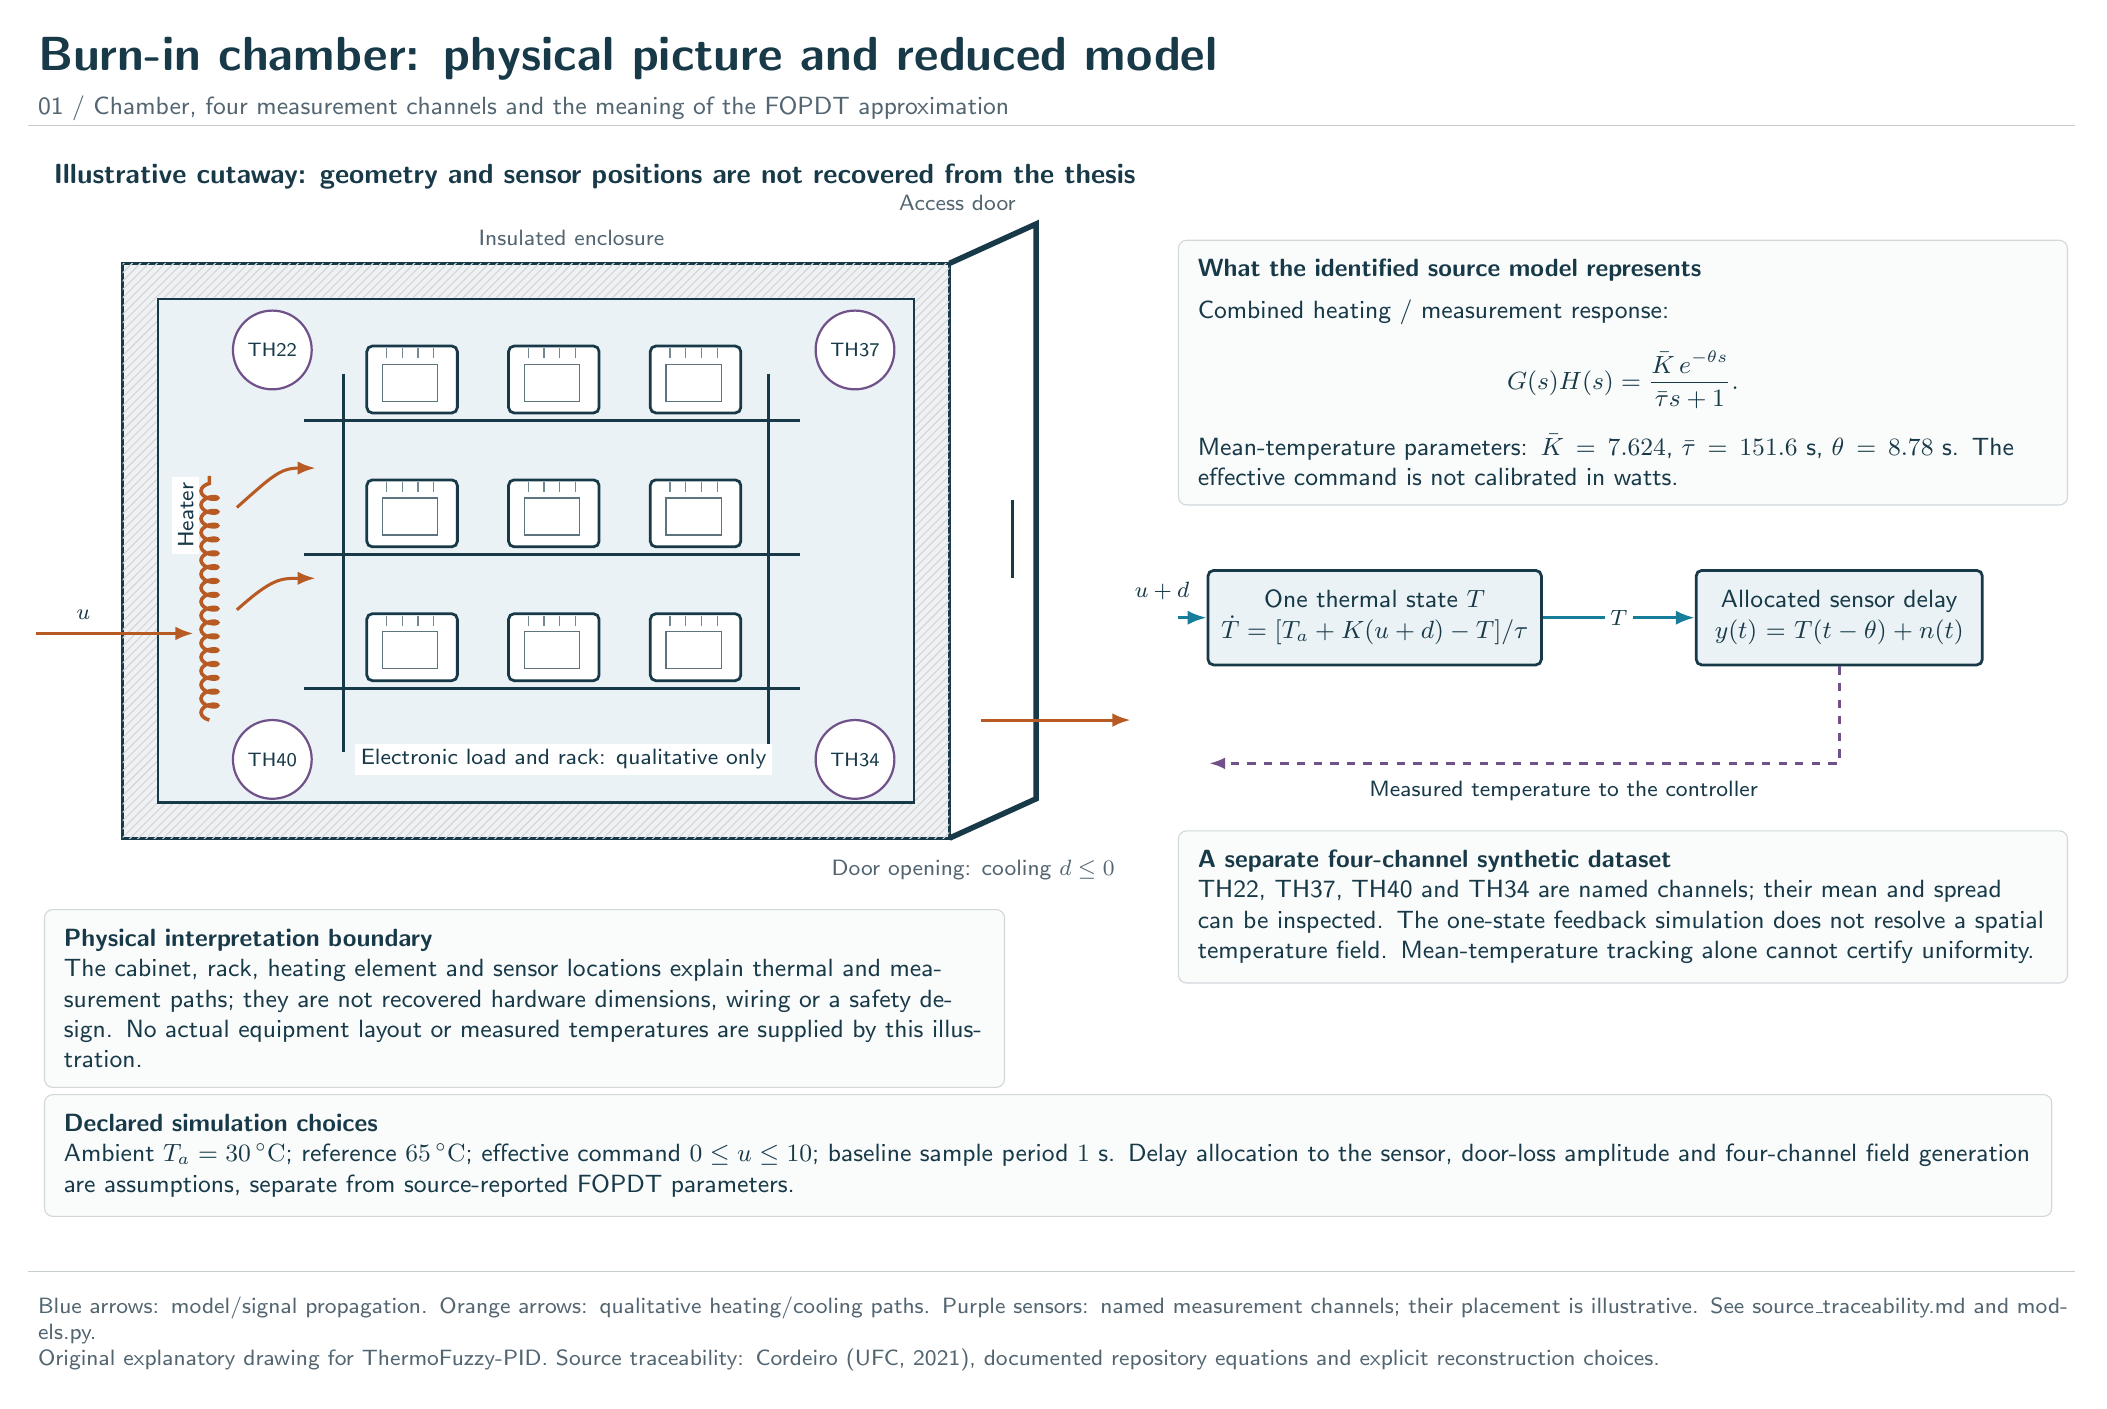
\begin{tikzpicture}[x=1cm,y=1cm]
\atlasheader{Burn-in chamber: physical picture and reduced model}{01 / Chamber, four measurement channels and the meaning of the FOPDT approximation}
\node[anchor=west,font=\sffamily\bfseries]at(.2,-1.9){Illustrative cutaway: geometry and sensor positions are not recovered from the thesis};
% Insulation, inner liner, door, rack and electronic load.
\path[draw=ink,line width=1.1pt,fill=ink!7](1.2,-3)rectangle(11.7,-10.3);
\path[pattern=north east lines,pattern color=ink!20](1.2,-3)rectangle(11.7,-10.3);
\path[draw=ink,fill=pale,line width=.9pt](1.65,-3.45)rectangle(11.25,-9.85);
\draw[ink,line width=2pt](11.7,-3)--(12.8,-2.5)--(12.8,-9.8)--(11.7,-10.3);
\draw[ink,line width=1.2pt](12.5,-6)--(12.5,-7);
\node[annotation,anchor=south]at(11.8,-2.45){Access door};
\draw[ink,line width=1pt](4,-4.4)--(4,-9.2)(9.4,-4.4)--(9.4,-9.2);
\foreach \yy in {-5.0,-6.7,-8.4}{
 \draw[ink,line width=1.2pt](3.5,\yy)--(9.8,\yy);
 \foreach \xx in {4.3,6.1,7.9}{
   \draw[equipment,fill=white](\xx,\yy+.1)rectangle(\xx+1.15,\yy+.95);
   \draw[ink!70](\xx+.2,\yy+.25)rectangle(\xx+.9,\yy+.72);
   \foreach \p in {.25,.45,.65,.85}{\draw[ink!60](\xx+\p,\yy+.8)--(\xx+\p,\yy+.92);}
 }
}
\node[labelbox]at(6.8,-9.3){Electronic load and rack: qualitative only};
\draw[heat,line width=1.3pt,decorate,decoration={coil,segment length=5pt,amplitude=3pt}](2.3,-8.8)--(2.3,-5.7);
\node[labelbox,rotate=90]at(2,-6.2){Heater};
\draw[thermal](.1,-7.7)--(2.1,-7.7);
\node[labelbox,anchor=south]at(.7,-7.6){$u$};
\draw[thermal](2.65,-6.1)..controls(3.1,-5.7)and(3.2,-5.6)..(3.65,-5.6);
\draw[thermal](2.65,-7.4)..controls(3.1,-7.0)and(3.2,-7.0)..(3.65,-7.0);
\node[annotation,anchor=south]at(6.9,-2.9){Insulated enclosure};
\foreach \xx/\yy/\name in {3.1/-4.1/TH22,10.5/-4.1/TH37,3.1/-9.3/TH40,10.5/-9.3/TH34}{
 \node[sensor,minimum size=10mm]at(\xx,\yy){\name};
}
\draw[thermal](12.1,-8.8)--(14,-8.8);
\node[annotation,anchor=north,align=center]at(12,-10.45){Door opening: cooling $d\le0$};
% Explicit mathematical boundary, separated from the illustrated spatial field.
\node[panel,anchor=north west,text width=10.8cm]at(14.6,-2.7){\textbf{What the identified source model represents}\\[4pt]
Combined heating / measurement response:
\[G(s)H(s)=\frac{\bar K\,e^{-\theta s}}{\bar\tau s+1}.\]
Mean-temperature parameters: $\bar K=7.624$, $\bar\tau=151.6$ s, $\theta=8.78$ s. The effective command is not calibrated in watts.};
\node[box,text width=4cm] (plant)at(17.1,-7.5){One thermal state $T$\\$\dot T=[T_a+K(u+d)-T]/\tau$};
\node[box,text width=3.4cm] (sensor)at(23,-7.5){Allocated sensor delay\\$y(t)=T(t-\theta)+n(t)$};
\draw[process](14.6,-7.5)--(plant.west);
\node[labelbox,anchor=south]at(14.4,-7.35){$u+d$};
\draw[process](plant.east)--node[labelbox]{$T$}(sensor.west);
\draw[signal](sensor.south)--(23,-9.35)--(15,-9.35);
\node[labelbox,anchor=north]at(19.5,-9.5){Measured temperature to the controller};
\node[panel,anchor=north west,text width=10.8cm]at(14.6,-10.2){\textbf{A separate four-channel synthetic dataset}\\TH22, TH37, TH40 and TH34 are named channels; their mean and spread can be inspected. The one-state feedback simulation does not resolve a spatial temperature field. Mean-temperature tracking alone cannot certify uniformity.};
\node[panel,anchor=north west,text width=11.7cm]at(.2,-11.2){\textbf{Physical interpretation boundary}\\The cabinet, rack, heating element and sensor locations explain thermal and measurement paths; they are not recovered hardware dimensions, wiring or a safety design. No actual equipment layout or measured temperatures are supplied by this illustration.};
\node[panel,anchor=north west,text width=25.0cm]at(.2,-13.55){\textbf{Declared simulation choices}\\Ambient $T_a=30\,^{\circ}\mathrm C$; reference $65\,^{\circ}\mathrm C$; effective command $0\le u\le10$; baseline sample period $1$ s. Delay allocation to the sensor, door-loss amplitude and four-channel field generation are assumptions, separate from source-reported FOPDT parameters.};
\atlasfooter{Blue arrows: model/signal propagation. Orange arrows: qualitative heating/cooling paths. Purple sensors: named measurement channels; their placement is illustrative. See source\_traceability.md and models.py.}
\end{tikzpicture}
\end{document}
